% !TeX root = ../sameplaper.tex
% !TeX spellcheck = en_US

\chapter{Homomorphic Encryption Deployment}
\setcounter{section}{0}

\section{HE deployment}
% Software that are used in real life applications face a variety of threats and challenges and also changes with the change of technology. A threat can arise form outside as well as from inside. An attacker can disable the system entirely or may get sensitive information from the system using the leakage of sensitive information leaked during computation. Result of this may result ino diminishing the users trust for the system. Thus threat modeling/analysis plays an important role to counter measure the threat from taking advantage of system design flaws resulting into leaking sensitive information. There are couple of threat modeling techniques available in the literature \cite{shevchenko_2018}. Identification of a suitable threat model for a particular application depend upon specific needs of the project.

Softwares that are used in real-life applications face a variety of threats and challenges and also changes with the change of technology. A threat can arise from outside as well as from inside. An attacker can disable the system entirely or may get sensitive information from the system using the system's leakage of sensitive information leaked during computation, which the attacker can use for financial gain or to disable the system altogether. This results in diminished users' trust in the system and may also result in considerable losses to the business. Thus, threat modeling or analysis plays an essential role in countering  system design flaws, which may result in the leakage of sensitive information. Several threat modeling techniques are available in the literature \cite{shevchenko_2018}. However, identifying a suitable threat model for a particular application depends on the project's specific needs.

Here we will use the STRIDE \cite{The_Threat_Model} model to investigate possible attacks in each entity/component and determine its mitigation techniques. By building a data flow diagram (DFD), STRIDE is used to view the system design details. STRIDE, a mnemonic of the terms Spoofing, Tempering, Repudiation, Information disclosure, Denial of Service, and Elevation of privilege, can be applied to any cyber-physical system. Figure \ref{fig:basic_dfd} shows the DFD drawn for studying STRIDE of HE deployment. As shown in the figure, each modular entity is considered separately, and its security and leakages are investigated individually.

Furthermore, deployment of HE can be divided into two parts. The first part focuses on creating a secure communication channel between the parties involved. For creating a secure communication channel between the user and the client query portal, we have suggested using public key infrastructure (PKI) \cite{PKI}. Figure \ref{fig_public_key_infrastructure} shows the use of PKI for secure electronic transfer of information of different kinds. PKI is usually required for activites where simple passwords are an inadequate authentication method and more rigorous proofs are required to confirm the identity of communicating parties involved so that some attacks like MITM can be avoided and to validate the information being transfered to the intended party.



%------------------------DFD starts here-------------------------------------------------
%Figure to show the TLS1.3 connection istablishment
\begin{figure}[!ht]
    \centering
    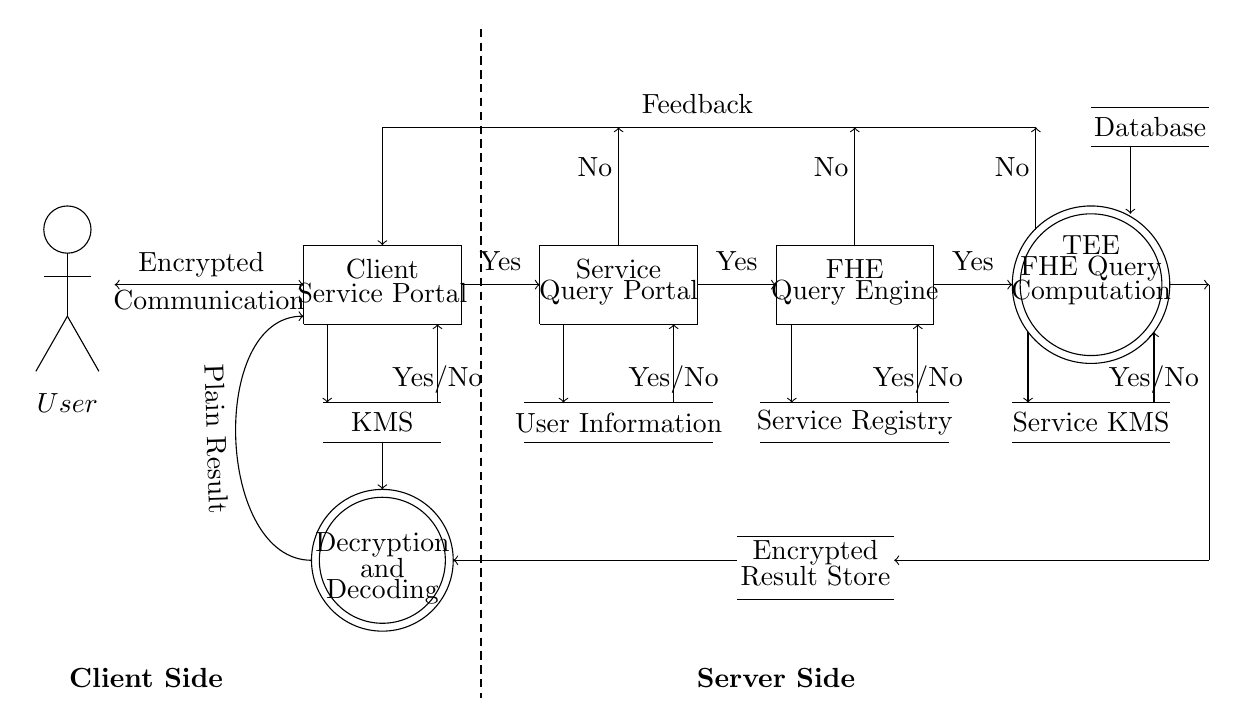
\begin{tikzpicture}

        %separating line between client and server
        \draw [thick , densely dashed] (-6.75,2.75) -- (-6.75,-5.75);
        \node at (-11,-5.5) {$\textbf{Client Side}$};
        \node at (-3,-5.5) {$\textbf{Server Side}$};

        %Drawing an User
        \draw (-12,.2) circle [radius=.3]; %head
        \draw (-12.3,-.4) -- (-11.7,-.4);  %hands .4 -.4   .7 .7
        \draw (-12,-.1) -- (-12,-.9); %spinal cord  0 0    .4 1.4
        \draw (-12,-.9) -- (-12.4,-1.6); %left leg 0 .4     1.4 2.2
        \draw (-12,-.9) -- (-11.6,-1.6); %right leg 0 -.5    1.4  2.2
        \node at (-12,-2) {$User$}; %0          -1.5


        % Client Service Portal
        \draw (-9,-1) -- (-7,-1) -- (-7,0) -- (-9,0) -- (-9,-1);
        \node at (-8,-.3) {Client };
        \node at (-8,-.6) {Service Portal};

        %connecting arrow between user and client query portal
        \draw [<->](-11.4,-.5) -- (-9,-.5);
        \node at (-10.3,-.25) {Encrypted};
        \node at (-10.2,-.7) {Communication};


        %KMS Database drawing
        \draw (-8.75,-2.5) -- (-7.25,-2.5);
        \draw (-8.75,-2) -- (-7.25,-2);
        \node at (-8,-2.25) {KMS};

        %Connecting line between KMS and client query portal
        \draw [<-](-8.7,-2) -- (-8.7,-1);
        \draw [->](-7.3,-2) -- (-7.3,-1);
        \node at (-7.3,-1.7) {Yes/No};

        %Connecting line between clent service portal and service query portal
        \draw [->](-7,-.5) -- (-6,-.5);
        \node at (-6.5,-.2) {Yes};


        % Service Query Portal
        \draw (-6,-1) -- (-4,-1) -- (-4,0) -- (-6,0) -- (-6,-1);
        \node at (-5,-.3) {Service };
        \node at (-5,-.6) {Query Portal};

        %User information Database drawing
        \draw (-6.2,-2.5) -- (-3.8,-2.5);
        \draw (-6.2,-2) -- (-3.8,-2);
        \node at (-5,-2.25) {User Information};

        %Connecting line between user information and service query portal
        \draw [<-](-5.7,-2) -- (-5.7,-1);
        \draw [->](-4.3,-2) -- (-4.3,-1);
        \node at (-4.3,-1.7) {Yes/No};

        %Connecting line between service query portal and FHE query engine
        \draw [->](-4,-.5) -- (-3,-.5);
        \node at (-3.5,-.2) {Yes};


        %FHE query engine
        \draw (-3,-1) -- (-1,-1) -- (-1,0) -- (-3,0) -- (-3,-1);
        \node at (-2,-.3) {FHE};
        \node at (-2,-.6) {Query Engine};

        %User Service registry Database drawing
        \draw (-3.2,-2.5) -- (-0.8,-2.5);
        \draw (-3.2,-2) -- (-.8,-2);
        \node at (-2,-2.25) {Service Registry};

        %Connecting line between FHE query engine and Service Registry
        \draw [<-](-2.8,-2) -- (-2.8,-1);
        \draw [->](-1.2,-2) -- (-1.2,-1);
        \node at (-1.2,-1.7) {Yes/No};

        %Connecting line between FHE query engine and TEE FHE query computation
        \draw [->](-1,-.5) -- (0,-.5);
        \node at (-.5,-.2) {Yes};

        %TEE FHE query computation
        \draw (1,-0.5) circle [radius=.9]; %head
        \draw (1,-0.5) circle [radius=1]; %head
        \node at (1,0) {TEE};
        \node at (1,-.3) {FHE Query};
        \node at (1,-.6) {Computation};

        %User Service KMS Database drawing
        \draw (0,-2.5) -- (2,-2.5);
        \draw (0,-2) -- (2,-2);
        \node at (1,-2.25) {Service KMS};

        %Connecting line between FHE query engine and Service Registry
        \draw [->](1.8,-2) -- (1.8,-1.1);
        \draw [<-](.2,-2) -- (.2,-1.1);
        \node at (1.8,-1.7) {Yes/No};

        %feedback system
        \draw []   (-8,1.5) -- (.3,1.5);
        \node at (-4,1.8) {Feedback};
        \draw [->]  (.3,.2) -- (.3,1.5); %TEE to line
        \node at (0,1) {No};

        \draw [->] (-2,0) -- (-2,1.5); %FHE query engine to line
        \node at (-2.3,1) {No};

        \draw [->] (-5,0) -- (-5,1.5); %Service query portal to line
        \node at (-5.3,1) {No};

        \draw [->] (-8,1.5) -- (-8,0); %Client Service portal to line



        %Database drawing
        \draw (1,1.75) -- (2.5,1.75);
        \draw (1,1.25) -- (2.5,1.25);
        \node at (1.75,1.5) {Database};
        \draw [->](1.5,1.25) -- (1.5,.4);

        %Computed Result send to Encrypted Result store
        \draw [<-](-1.5,-4)  -- (2.5,-4);
        \draw [-](2.5,-4) -- (2.5,-.50);
        \draw [<-](2.5,-.50)    -- (2,-.5);
        \draw [->](-3.5,-4)  -- (-7.1,-4);

        %Computed store in temporary database
        \draw (-1.5,-3.70) -- (-3.5,-3.70);
        \draw (-1.5,-4.5) --  (-3.5,-4.5);
        \node at (-2.5,-3.9) {Encrypted};
        \node at (-2.5,-4.2) {Result Store};


        %TEE computation
        \draw (-8,-4) circle [radius=.8]; %head
        \draw (-8,-4) circle [radius=.9]; %head
        \node at (-8,-3.8) {Decryption};
        \node at (-8,-4.1) {and};
        \node at (-8,-4.4) {Decoding};

        %Line from KMS to the Decryption and Decoding
        \draw [<-](-8,-3.1) --  (-8,-2.5);

        %Connecting line between decryption and decoding and client service portal
        \draw [ <- ] (-9,-.9)  to  [out=180, in=180  ,edge node={node [sloped,below]  {Plain Result}}] (-8.9,-4) ;




    \end{tikzpicture}
    \caption{Basic data flow diagram of FHE query computation}
    \label{fig:basic_dfd}
\end{figure}
%------------------------DFD ends here-------------------------------------------------
% \begin{figure}
%   \includegraphics[width=1.2\linewidth]{Diagrams/Basic_DFD.png}
%   \caption{Basic data flow diagram of FHE query computation}
%   \label{fig:basic_dfd}
% \end{figure}
%-------------------------------------------------------------------------------------


%------------------------PKI starts here onwards-------------------------------------------------
%Figure to show the TLS1.3 connection istablishment
\begin{figure}[!ht]
    \centering
    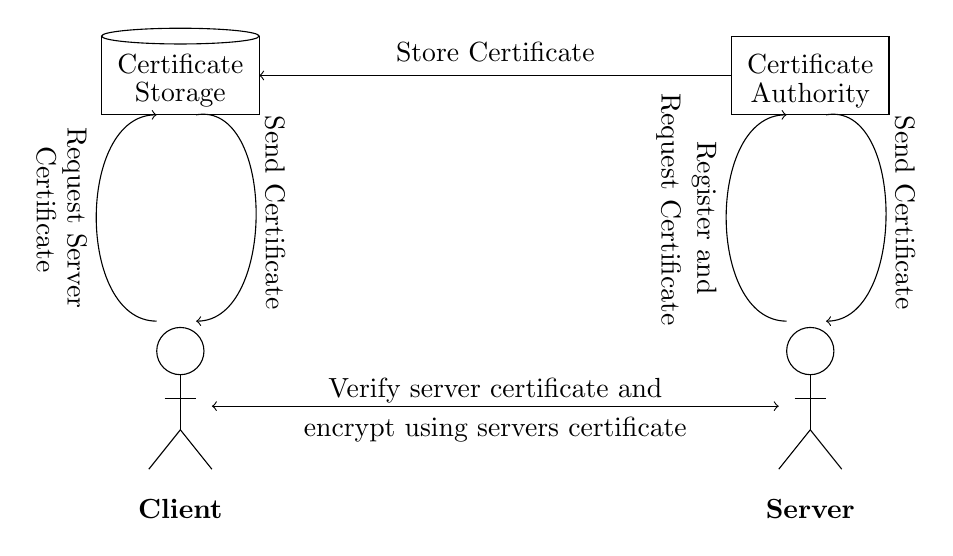
\begin{tikzpicture}

        %Drawing Client
        \draw (-12,0) circle [radius=.3]; %head
        \draw (-12.2,-.6) -- (-11.8,-.6);  %hands .4 -.4   .7 .7
        \draw (-12,-.3) -- (-12,-1); %spinal cord  0 0    .4 1.4
        \draw (-12,-1) -- (-12.4,-1.5); %left leg 0 .4     1.4 2.2
        \draw (-12,-1) -- (-11.6,-1.5); %right leg 0 -.5    1.4  2.2
        \node at (-12,-2) {$\textbf{Client}$}; %0          -1.5

        %Drawing Server
        \draw (-4,0) circle [radius=.3]; %head
        \draw (-4.2,-.6) -- (-3.8,-.6);  %hands .4 -.4   .7 .7
        \draw (-4,-.3) -- (-4,-1); %spinal cord  0 0    .4 1.4
        \draw (-4,-1) -- (-4.4,-1.5); %left leg 0 .4     1.4 2.2
        \draw (-4,-1) -- (-3.6,-1.5); %right leg 0 -.5    1.4  2.2
        \node at (-4,-2) {$\textbf{Server}$}; %0          -1.5

        %Connecting line between client and server x
        \draw [<->](-11.6,-.7) -- (-4.4,-.7);
        \node at (-8,-.5) {Verify server certificate and};
        \node at (-8,-1) {encrypt using servers certificate};


        %Certificate storage
        \draw (-13,3) -- (-11,3) -- (-11,4)  (-13,4) -- (-13,3);
        \draw (-12,4) ellipse (1cm and .1cm);
        \node at (-12,3.65) {Certificate};
        \node at (-12,3.25) {Storage};

        %Certificate authority
        \draw (-5,3) -- (-3,3) -- (-3,4) -- (-5,4) -- (-5,3);
        % \draw (-12,4) ellipse (1cm and .1cm);
        \node at (-4,3.65) {Certificate};
        \node at (-4,3.25) {Authority};

        %Line between certificate storage and Certificate Authority
        \draw [<-](-11,3.5) -- (-5,3.5);
        \node at (-8,3.8) {Store Certificate};

        %Line between Server and Certificate Authority
        % \draw [<->](-4,3) -- (-4,.4);

        %Connecting line between certificate storage and client
        % \draw [<->](-12,.4) -- (-12,3);

        %Connecting line between server and certificate authority
        \draw [ <- ]  (-12.3,3) to  [out=180, in=180  ,edge node={node [sloped,below]  {Request Server}}] (-12.3,.38);
        \node at (-13.7,1.8) [rotate=270] {Certificate};
        \draw [ -> ]  (-11.8,3) to  [out=10 , in=360 ,edge node={node [sloped,above]   {Send Certificate}}] (-11.8,.38);


        %Connecting line between server and certificate authority
        % \path (2,1,0)
        \node at (-5.8,1.8) [rotate=270] {Request Certificate};
        \draw [ <-]  (-4.3,3) to  [out=180, in=180  ,edge  node={node [sloped,below]  {Register and}}] (-4.3,.38);
        \draw [ ->]  (-3.8,3) to  [out=10 , in=360  ,edge  node={node [sloped,above]  {Send Certificate}}] (-3.8,.38);

    \end{tikzpicture}
    \caption{Public key infrastructure}
    \label{fig_public_key_infrastructure}
\end{figure}
%------------------------PKI ends here-------------------------------------------------



The PKI used to achieve a secure communication channel can be either TLS1.2 or TLS1.3. However, in our case, we have assumed using LTS1.3 as it provides optimal secure channel creation time. Different steps to create a secure communication channel between the user and the client query portal using TLS1.3 is shown in figure \ref{TLS1.3_handshake}. A more detailed description about TLS1.3 can be obtained in \cite{TLS13}.




%------------------------------------------------------Handshaking protocol in TLS 1.3-------------------------------------------------
\begin{figure}[!ht]
    \centering
    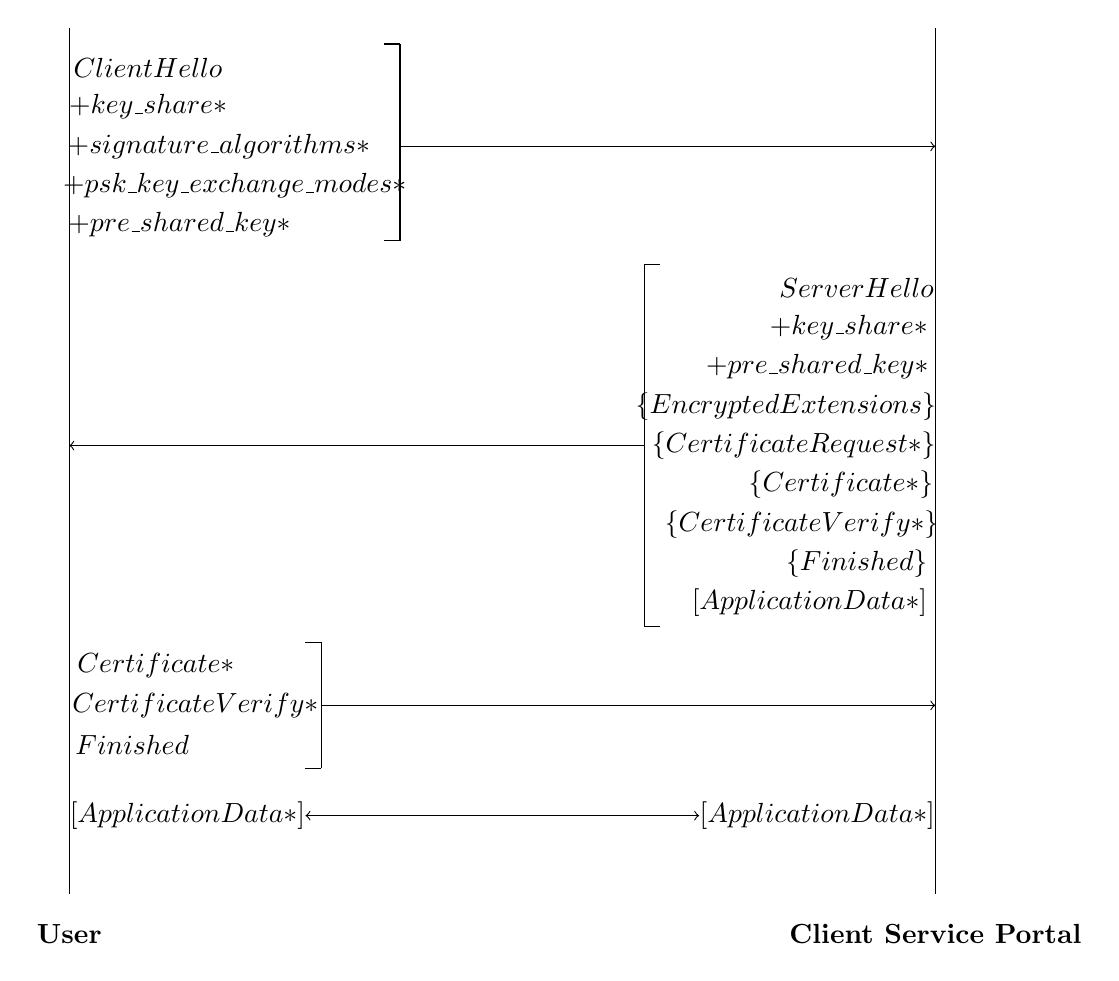
\begin{tikzpicture}

        \node at (-11,-5.5) {$\textbf{User}$}; %0          -1.5
        \node at (0,  -5.5) {$\textbf{Client Service Portal}$}; %0          -1.5

        %client line
        \draw (-11,6) -- (-11,-5);

        %Server line
        \draw (0,6) -- (0,-5);

        %client lessages
        %key exchange
        % \node at (-10,5.5)   {$ClientHello$};

        %---------------------
        \draw (-6.8,5.8) -- (-6.8,3.3);
        \draw (-7,5.8) -- (-6.8,5.8);
        \draw (-7,3.3) -- (-6.8,3.3);
        \node at (-10,5.5)   {$ClientHello$};
        \node at (-10,5)     {$+ key\_share*$};
        \node at (-9.1,4.5)   {$+ signature\_algorithms*$};
        \node at (-8.9,4)     {$+ psk\_key\_exchange\_modes*$};
        \node at (-9.6,3.5)   {$+ pre\_shared\_key*$};
        \draw[->] (-6.8,4.5) -- (0,4.5);


        %Server messages
        \draw (-3.7,   3) -- (-3.7,-1.6);
        \draw (-3.7,   3) -- (-3.5,   3);
        \draw (-3.7,-1.6) -- (-3.5,-1.6);


        \node at (-1,2.7)   {$ServerHello$};
        \node at (-1.1,2.2)   {$+ key\_share*$};
        \node at (-1.5,1.7)   {$+ pre\_shared\_key*$};
        \node at (-1.9,1.2)   {$\{EncryptedExtensions\}$};
        \node at (-1.8,.7)   {$\{CertificateRequest*\}$};
        \node at (-1.2,.2)   {$\{Certificate*\}$};
        \node at (-1.7,-.3)   {$\{CertificateVerify*\}$};
        \node at (-1,-.8)   {$\{Finished\}$};
        \node at (-1.6,-1.3)   {$[Application Data*]$};
        \draw[<-] (-11,.7) -- (-3.7,.7);

        %clent messages
        \draw (-7.8,-1.8) -- (-7.8,-3.4);
        \draw (-8,-3.4) -- (-7.8,-3.4);
        \draw (-8,-1.8) -- (-7.8,-1.8);
        \node at (-9.9,-2.1)   {${Certificate*}$};
        \node at (-9.4,-2.6)     {${CertificateVerify*}$};
        \node at (-10.2,-3.1)   {${Finished}$};
        \draw[->] (-7.8,-2.6) -- (0,-2.6);

        %communication start
        \node at (-9.5,-4)   {$[Application Data*]$};
        \node at (-1.5,-4)   {$[Application Data*]$};
        \draw[<->] (-8,-4) -- (-3,-4);

    \end{tikzpicture}
    \caption{TLS 1.3 Handshake. In the figure $+$ Indicates noteworthy extensions sent in the previously noted message. $*$ Indicates optional or situation-dependent messages/extensions that are not always sent. $\{\}$ Indicates messages protected using keys derived from a [sender]$\_$handshake$\_$traffic$\_$secret. $[]$ Indicates messages protected using keys derived from [sender]$\_$application$\_$traffic$\_$secret$\_N$.}
    \label{TLS1.3_handshake}
\end{figure}
%-------------------------------------------------------------------------------------------------------




\begin{comment}
%Figure to show the TLS1.3 connection istablishment
\begin{figure}[!ht]
    \centering
    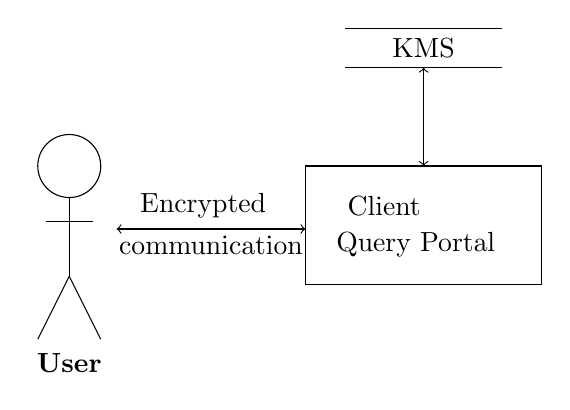
\begin{tikzpicture}

        %Drawing an User
        \draw (-12,0) circle [radius=.4]; %head
        \draw (-12.3,-.7) -- (-11.7,-.7);  %hands .4 -.4   .7 .7
        \draw (-12,-.4) -- (-12,-1.4); %spinal cord  0 0    .4 1.4
        \draw (-12,-1.4) -- (-12.4,-2.2); %left leg 0 .4     1.4 2.2
        \draw (-12,-1.4) -- (-11.6,-2.2); %right leg 0 -.5    1.4  2.2
        \node at (-12,-2.5) {$\textbf{User}$}; %0          -1.5

        % Service Query Portal
        \draw (-9,-1.5) -- (-6,-1.5) -- (-6,0) -- (-9,0) -- (-9,-1.5);
        \node at (-8,-.5) {Client};
        \node at (-7.6,-1) {Query Portal};

        %Database drawing
        \draw (-8.5,1.75) -- (-6.5,1.75);
        \draw (-8.5,1.25) -- (-6.5,1.25);
        \node at (-7.5,1.5) {KMS};

        %connecting arrow between user and client query portal
        \draw [<->](-11.4,-.8) -- (-9,-.8);
        \node at (-10.3,-.5) {Encrypted};
        \node at (-10.2,-1) {communication};

        %Connecting line between KMS and client query portal
        \draw [<->](-7.5,1.25) -- (-7.5,0);

    \end{tikzpicture}
    \caption{Interaction between user and the client query portal}
    \label{fig_user_Client_query_portal_interactions}
\end{figure}
\end{comment}






Once the key materials are shared using TLS $1.3$, all followed interactions are performed using the cryptographic parameters shared during the TLS handshake protocol in the encrypted domain as depicted by figure \ref{fig:basic_dfd}. TLS handshake protocol allows both parties to negotiate a protocol version, select cryptographic algorithms, optionally authenticate each other and establish shared secret keying material. Once handshaking is complete, parties use the specified keys to protect the application-layer data. Failure of the handshake or other protocol triggers termination of the connection, optionally preceded by an alert message.


%and tried to mitigate anomalies observed.
When a client performs secure authentication using his credentials, viz username, and password, he can use the registered services available for the users. However, it is emphasized that the query encryption key is never shared with the user. The user's query is encrypted in the client service portal using the standard methods present in the client service portal. By doing so, use of more errors for query encryption for an intentional decryption failure attack can be safely restricted. Additionally, there needs to be more than encrypted communication between the user and the client service portal to ensure secure query encryption. The user, as well as the client service portal, may be malicious and may act as an active or passive attacker. Thus all possible behavior of the user and client service portal must be analyzed, and its mitigation techniques must be suggested. Below, we have performed a case study on the user and the client service portal based on their behavior.

The user's query can be sent for computation to the query service portal in two different ways. Each of these has its associated advantage and shortcomings. Either of these techniques is implementation specific and decided based on project requirements. In our case, we suggest using the second technique for HE deployment.

In the first technique, a user query is sent with user metadata for query computation. In this case, the user's authentication is performed using the user database stored in the server, and the same is true for the service validity check. After successful authentication and verification, the query computation is performed, which is decrypted and decoded, and the obtained final plain result is forwarded to the user who submitted the query. This method requires maintenance of the user's database on the server side. Similarly, the user's service information must be stored on the server side for a service check. As more users register with the institutions, they must constantly update and maintain the database. Similarly, when a user's registration has been withdrawn, it has to be updated on the server side, which creates a heavy overload on the server side.

In the second technique, the user's query is sent with the institution's metadata. When a user asks for a query request, the user's authentication is verified in the client-side portal. On successful authentication, the user's queries are sent with the institution's metadata storing the user's information requesting the service on the client-side portal, specifically in the service request database. The server side performs institution authentication and service validation of the institution. On successful authentication and service request verification, query computation is performed. The result is forwarded to the institution. The institution identifies the user who generated the query request from the service request database and sends the query result to the corresponding query user.



\newpage

\section{Client Side Security Analysis: Secure communication}
\label{possible-attacks_in_components}

\subsection{User}
\begin{itemize}
    \item An unauthorized user tries to access the services
          \begin{itemize}
              \item To access services the user needs to be registered; upon registration, login credentials are provided to the user.
              \item Unless the user has the login credentials of a registered user, he can not access the services.
              \item Upon registration user gets the signing key that he uses for creating query signature and send with query.
          \end{itemize}

    \item A user uses brute force to guess login credentials of registered user
          \begin{itemize}
              \item These types of attacks can be restricted by using an additional layer of authentication in the form of multifactore authenticator to use the facility.
              \item However, during implementation, it needs to be ensured that the user's credentials are verified only after multifactore authentication.
              \item On successful multifactore authentication, user's credentials are verified a threshold number of times, and after that user may be blocked for a specific time interval based on the security requirements.
          \end{itemize}

    \item An attacker may try to steal the login information of the user by social engineering or by impersonation attack (attempt to gain unauthorized access to systems by masquerading as authorized users)
          \begin{itemize}
              \item As mentioned above, these attacks can be restricted using an additional layer of authentication in the form of multifactore authentication.
          \end{itemize}

    \item Attackers may eavesdrop on the communication link, modify the communicated data or prevent communication between the user and the client service portal
          \begin{itemize}
              \item As mentioned above, the user and client service portal communicates using a secure communication channel built using TLS1.3. Thus eavesdropping on the communication link between the user and the client service portal is restricted by TLS1.3.
          \end{itemize}

    \item User uses feedback mssages to gain secret information about the system
          \begin{itemize}
              \item Feedback messages do not reveal any secret information to the user by design. It will be clear when we discuss the feedback messages sent to the user.
          \end{itemize}
    \item A genuine user forgets his password
          \begin{itemize}
              \item On successful completion of multifactor authentication user is taken to the password reset page where he can reset his password
          \end{itemize}
    \item User revocation by institution
          \begin{itemize}
              \item In such cases, user can not pass the client service portal
              \item This must be easy to implement and operate
          \end{itemize}
\end{itemize}


\subsection{Client Service Portal}

Clent service portal can be further divided into two categories: Compromised and Passive Attacker. Below we will study security threats posses to the system by each of these categories.
\subsubsection{Passive Attacker}
\begin{itemize}
    \item Denial of service attack
          \begin{itemize}
              \item The user cannot perform any query on the database.
              \item The reason is mentioned in the feedback reply sent to the user with the standard error code.
          \end{itemize}
    \item The authorization of an unauthorized user
          \begin{itemize}
              \item This situation may arise when a user is completely compromised.
              \item An attacker with the key and metadata of a genuine user can’t be detected, provided he has access to the multifactor authenticator.
              \item Thus, he can perform query computation without any problem and finally gets the result as a regular genuine user.
              \item However, this type of attack can be avoided by sending a feedback reply to the user on user login. If he is not the one into the system then he is suggested to change his credentials immediately.
          \end{itemize}

    \item Institution revocation by Service Query Portal
          \begin{itemize}
              \item Institution can not perform any query operation
              \item This operation must be easy to implement and operate
          \end{itemize}

\end{itemize}

\subsubsection{Compromised}
\begin{itemize}
    \item Genuine user authentication failure
          \begin{itemize}
              \item The user cannot login to the client service portal the perform query on the database.
              \item However, the user knows why the authentication failed through the feedback received.
              \item The feedback sent has the reason behind the authentication failure as a standard error code like user credentials are incorrect.
          \end{itemize}
    \item The requested service was not provided to the user
          \begin{itemize}
              \item The user cannot perform the intended service computation on the database.
              \item The reason is mentioned with a standard error code in the feedback reply. Thus the user knows the reason behind the requested service failure.
          \end{itemize}

          %         \item Client Service Portal can send (encryption key, metadata) in the following four possible ways
          %
          %             \begin{itemize}
          %                 \item Correct, Correct
          %                 \begin{itemize}
          %                     \item This is correct and creates no problem for query computation
          %                 \end{itemize}
          %                 \item Correct, Wrong
          %                 \begin{itemize}
          %                     \item Wrong here means metadata is of another user
          %                         (If metadata is completely wrong, then it gets detected in the service query portal when user is verified)
          %                     \item The user encrypts his query and sends it for query computation
          %                     \item Service query portal authenticates the user and sends it to FHE Query Engine
          %                     \item Service registry authenticates the user if it has access for the service requested then he replies with the user metadata
          %                     \item The service key is asked from service KMS using user’s metadata and service KMS replies with necessary keys
          %                     \item FHE query engine performs query computation and stores it in the encrypted form
          %                     \item Encrypted result is decrypted in the TEE and later it is sent to the user.
          %                     \item However, the result obtained by the user is wrong due to wrong key used for query encryption in the first place itself.
          %                     \item \textcolor{blue} {I think this form of attack can be restricted by storing metadata and key along with its DS}.
          %                 \end{itemize}
          %                 \item Wrong , Correct
          %                 \begin{itemize}
          %                     \item Using the same techniques as that of above this form of attack can be identified and restricted
          %                 \end{itemize}
          %                 \item Wrong, Wrong
          %                 \begin{itemize}
          %                     \item He gets detected in the service query portal when the user gets verified
          %                 \end{itemize}
          %             \end{itemize}


    \item The query malleability
          \begin{itemize}
              \item Query encryptions are performed in three steps in the order: encoding, encryption, and signature computation.
              \item Query encryption is performed in the TEE environment in the client service portal.
              \item Before query encryption query malleability check is performed inside the TEE environment. On successful query signature validation, query encoding is performed, followed by query encryption.
              \item Query signature computation is performed upon query encryption.
              \item Finally, the obtained encrypted query and query signature is sent to Service Query Portal for query computations.
              \item Query malleability on transit can be restricted by using TLS1.3 by creating a secure communication channel.+6
          \end{itemize}
\end{itemize}


\section{Server Side Security Analysis: HE Computation}

In the second part security of homomorphic computation is taken care of. In this part, all communication performed by the client query portal having encrypted query to obtain a query answer and homomorphic computation is handled. In the process, if any entity leaks any sensitive information, it is analyzed, and mitigation techniques are suggested to avoid such attacks or leakages. For completeness of risk analysis, we will consider each entity individually, considering what information is available to the entity and, using that, what kind of security threat the entity may pose to the system if the entity behaves as a passive or as an active attacker. We will also consider what kind of secret information the system may leak as a whole and by each entity during HE computation and try to suggest technologies that can be used to avoid such leakages.


%----------------------------------------------------
\label{possible-attacks_in_components}

\subsection{Service Query Portal}
\begin{itemize}
    \item Denial of service attack
          \begin{itemize}
              \item Institution cannot perform any query on the database
              \item However, this can be avoided using standard techniques of overcoming denial of service attack
          \end{itemize}
    \item Authorization failure attack
          \begin{itemize}
              \item The institution cannot perform any query on the database
              \item However, the same is conveyed to the institution by a standard error code as a feedback message sent.
          \end{itemize}
    \item Query malleability attack
          \begin{itemize}
              \item The query service portal can perform query malleability
              \item However, this can be avoided by sending digital signature of the encrypted query along with the query.
          \end{itemize}
    \item Query id malleability attack
          \begin{itemize}
              \item If the query id is modified, then it produces results, but the genuine user can’t fetch the result in the final step.
              \item However, this can be restricted by including the Institutional id, user id, and job id in the digital signature computation by the client service portal.
              \item Thus, by checking the digital signature, the query is dropped with a standard message sent back to the user if any discrepancy is found.
          \end{itemize}
    \item Incorrect digital signature received from the client query portal
          \begin{itemize}
              \item Service query portal discards the query if digital signature check fails
              \item Sends feedback to the user with a standard error message representing digital signature check fail.
          \end{itemize}
\end{itemize}
\subsection{Service Registry}
\begin{itemize}
    \item Denial of service attack
          \begin{itemize}
              \item Institution are not allowed to perform any query on the database
              \item This can be avoided by using standard techniques of overcoming denial of service attacks
          \end{itemize}
    \item Service authentication fail
          \begin{itemize}
              \item Query discarded from further processing
              \item However, the institution is informed by sending feedback message with standard error code representing service authentication fail
          \end{itemize}
    \item Service registry sends incorrect user metadata (Service Id, Service Name, HE Parameters, HE Client)
          \begin{itemize}
              \item This kind of discrepancies can be avoided by storing digital signature computed as DS(Institution Id + Service Id + Service name + HE Parameters + HE Client)
              \item Thus, when TEE gets the service parameters (Service Id, Service Name, HE Parameters, HE Client) from Service Registry and query information (Institution Id + Service Id + Service name) from query metadata. It computed the signature and verifies that it has indeed received the correct service parameters.
              \item If the computed DS do not match with that of the obtained DS, then he can perform either of the following two operation
                    \begin{itemize}
                        \item He can either ask for service parameters from service registry or
                        \item He can send feedback to the institution a stand error code representing service parameter check fail
                    \end{itemize}
          \end{itemize}
\end{itemize}

\subsection{Service Key Management System}
\begin{itemize}
    \item Denial of service attack
          \begin{itemize}
              \item Query processing not allowed to perform on the database
              \item This can be avoided using standard techniques of overcoming denial of service attack
          \end{itemize}
    \item Key malleability attack
          \begin{itemize}
              \item This can be avoided by storing Public key and Evaluation key encrypted with HSM using symmetric key encryption like AES with its digital signature.
              \item Digital signature here is computed as DS(Institution Id + HSM(Public Key) + HSM(Evaluation Key))
              \item TEE performs DS check if any inconsistency is observed
                    \begin{itemize}
                        \item It either requests the service key from service key management system or
                        \item Sends feedback to the institution with standard error code.
                    \end{itemize}
          \end{itemize}
    \item Wrong key Sent
          \begin{itemize}
              \item As mentioned above, the digital signature can be used to check whether the service key management system has sent the wrong key. If so, then appropriate action is taken.
          \end{itemize}
\end{itemize}

\subsection{Database}
\begin{itemize}
    \item Denial of service attack
          \begin{itemize}
              \item Query processing not allowed to perform on the database
              \item This can be avoided by using standard techniques of overcoming denial of service attack
          \end{itemize}
    \item Decryption failure due to wrong data provided for computation
          \begin{itemize}
              \item This type of attacks can be avoided by encrypting database using the attestation key of TEE.
          \end{itemize}
\end{itemize}

\subsection{FHE Query Computation}
\begin{itemize}
    \item Denial of service attack
          \begin{itemize}
              \item Query processing not allowed to perform on the database
              \item This can be avoided by using standard techniques of overcoming DOS
          \end{itemize}
    \item Decryption failure attack due to different circuit computation
          \begin{itemize}
              \item Query is feed along with its digital signature to the TEE
              \item TEE computes digital signature of the query and checks to find out correct circuit has been provided for the computation
              \item If incorrect circuit has been provided for computation, then sends feedback to the user with standard error message.
              \item Thus, this type of attack can be avoided by computing and verifying digital signature inside TEE
          \end{itemize}
    \item Query result malleability attack
          \begin{itemize}
              \item FHE Query Engine can modify the query result
              \item However, this can be restricted by computing query result digital signature in the TEE itself before providing it to FHE Query Engine.
              \item Send both encrypted query result and signature to the encrypted result store
          \end{itemize}
    \item Side channel attack
          \begin{itemize}
              \item Side channel attack can be avoided by computing query result in the TEE
          \end{itemize}
    \item Known plaintext attack (computation performed in plaintext domain)
          \begin{itemize}
              \item  Same as that of the above i.e., computation performed in the TEE
          \end{itemize}
\end{itemize}

\subsection{Decryption and Decoding}
\begin{itemize}
    \item Denial of service attack
          \begin{itemize}
              \item User denied from fetching query result.
              \item However, this can be avoided using standard techniques of overcoming DOS
          \end{itemize}
    \item Query result malleability attack
          \begin{itemize}
              \item TEE before decryption computes signature and checks its integrity with that of the signature received from the FHE Query Engine
              \item If case of any discrepancy, send feedback to the query service portal stating query integrity breached
          \end{itemize}
    \item Decryption failure attack
          \begin{itemize}
              \item If decryption fail is obtained, then it must be genuine and, in such scenario, the obtained result is sent to the User.
          \end{itemize}
    \item Side channel attack
          \begin{itemize}
              \item Decryption of the encrypted query result is performed in the TEE thus avoiding the side channel attack
              \item Also, TEE directly send the decrypted query result to user using HTTPS connection avoiding further attacks while query result is in transit.
          \end{itemize}
\end{itemize}


